
\chapter{SST Forcing}
\lastupdated{2024-11-30 15.52 }{\chapterSixSSTForcingOverleaf}

Understanding SST variability and its role in shaping atmospheric anomalies is essential for seasonal climate forecasting. For example:
\begin{itemize}
	\item Accurate SST forecasts for the next six months could provide critical insights into the likelihood of large-scale phenomena like El Niño, monsoons, or droughts, which are influenced by SST variability.
	\item Coupled ocean-atmosphere models that incorporate both internal dynamics and external SST-driven responses are critical for advancing our ability to predict climate anomalies over seasonal to interannual timescales.
\end{itemize}


One of the primary ways climate forcing impacts SSTs is through changes in radiative energy balance. For instance, increasing greenhouse gas concentrations trap outgoing longwave radiation, causing the Earth’s surface, including the oceans, to warm. Oceans absorb more than 90\% of this excess heat, resulting in widespread SST increases. The effects are not uniform, as ocean dynamics influence regional variations in warming. For example, the Western Pacific Warm Pool retains more heat due to strong stratification, while upwelling regions, such as the eastern Pacific, may experience slower warming due to the cooling effects of vertical mixing and horizontal ocean currents.

Other forms of climate forcing also influence SSTs. Volcanic aerosols and human-emitted sulfate aerosols, for example, reflect incoming solar radiation, leading to localized or even global cooling of SSTs. The cooling effects are often more pronounced in the Northern Hemisphere, where industrial activity has historically been concentrated. In contrast, variations in solar radiation cause more subtle, global SST changes due to the ocean’s high heat capacity.

\paragraph{SST Changes as Feedback to Climate Forcing.}
SST changes resulting from climate forcing do not only respond passively but also act as drivers of feedback mechanisms that amplify or modulate the effects of climate forcing. A key example is the water vapor feedback. Warmer SSTs increase evaporation rates, introducing more water vapor into the atmosphere. Since water vapor is a potent greenhouse gas, this enhances warming further. Similarly, SST changes influence cloud formation, which can either reflect sunlight back to space (cooling the Earth) or trap outgoing heat (warming the Earth). The balance of these cloud feedbacks is a significant area of ongoing research.


SST changes driven by climate forcing also amplify or modify major climate phenomena. One well-known example is the El Niño-Southern Oscillation (ENSO). Global warming is thought to alter SST patterns in the tropical Pacific, potentially affecting the frequency or intensity of El Niño and La Niña events. For instance, by flattening the SST gradient between the eastern and western Pacific, warming may weaken the Walker Circulation and favor more frequent El Niño-like conditions. Such shifts have significant implications for global rainfall patterns, droughts, and extreme weather events.

Changes in SSTs also influence large-scale ocean circulation patterns, such as the Atlantic Meridional Overturning Circulation (AMOC). Climate forcing that warms SSTs in the North Atlantic can disrupt this critical current system, leading to cascading effects on regional climates, including shifts in monsoons and weather systems across Europe and North America.

Long-term observations provide clear evidence of the impact of climate forcing on SSTs. Since the late 19th century, global SSTs have risen by approximately 0.8°C, primarily driven by greenhouse gas emissions. However, the warming is not evenly distributed. For example, the Arctic Ocean has experienced significantly faster warming due to the ice-albedo feedback, where melting ice exposes darker ocean surfaces that absorb more solar energy. Meanwhile, regions with persistent upwelling, such as the coast of Peru, have shown slower warming because cooler waters are constantly brought to the surface from the deep ocean.


From greenhouse gases, aerosols, or volcanic activity—can alter the strength and structure of the Walker Circulation by modifying the SST patterns or atmospheric stability.
ENSO Events (a result of internal variability but influenced by external forcing): El Niño events weaken the Walker Circulation as warm SST anomalies dominate the central and eastern Pacific; La Niña events strengthen it as cooler SSTs enhance upwelling in the east and convection in the west.
Observational studies found the importance of SST in the forcing of atmospheric anomalies.


\section{How can surface sea temperature impact atmospheric circulation?}

Let's consider the vorticity equation
\begin{equation}\label{eq. 2.1}
	\frac{\partial \zeta}{\partial t} = - \nabla \cdot (\zeta + f) \mathbf{V} = - (\zeta + f) \nabla \cdot \mathbf{V} - \mathbf{V} \cdot \nabla (\zeta + f) = - (\zeta + f) D - \mathbf{V} \cdot \nabla (\zeta + f)
\end{equation}

In equation \ref{eq. 2.1} D is the divergence and it is equal to
\begin{equation}
	D=u_x + v_y = w_z = \frac{\partial w}{\partial z}
\end{equation}
and the last term is the advection.


If we linearize \ref{eq. 2.1}, all the nonlinear terms will be thrown away so that
\begin{equation}\label{eq 2.3}
	\frac{\partial \zeta}{\partial t} = - f D - v \frac{\partial f}{\partial y} = - f D - \beta v
\end{equation}
\begin{equation}
	\frac{\partial \zeta}{\partial t} = - f \frac{\partial w}{\partial z} - \beta v
\end{equation}

The equation \ref{eq 2.3} stresses that vorticity evolves due to these two terms.
Assuming steady motion
\begin{equation}
	f \frac{\partial w}{\partial z} = \beta v
\end{equation}

What about the atmosphere?
We need to use a shallow water equation centered at the equation, this means in beta plane approximation.

\begin{equation}
	u_z- fv = -g \frac{\partial u}{\partial x}
\end{equation}

\begin{equation}
	v_z + fu = -g \frac{\partial u}{\partial y}
\end{equation}

So that
$$-\beta_y v = -g \frac{\partial h}{\partial x} + \frac{X}{\rho H}$$
$$\beta_y u = -g \frac{\partial h}{\partial y} + \frac{Y}{\rho H}$$
$$c^2 (u_x + v_y) = -\frac{gE}{\rho}$$
where X, Y, and E are external forcing terms.
These equations are not in balance because I need to add dissipation representing the effects of nonlinear terms.
\begin{equation}\label{eq 2.8}
	r u - \beta_y v = -g \frac{\partial h}{\partial x} + \frac{\rho H}{X}
\end{equation}


\begin{equation}\label{eq 2.9}
	r v +\beta_y u = -g \frac{\partial h}{\partial y} + \frac{Y}{\rho H}
\end{equation}

\begin{equation}\label{eq 2.10}
	r g h + c^2 (u_x + v_y) = -\frac{gE}{\rho}
\end{equation}



These equations \ref{eq 2.8}, \ref{eq 2.9}, \ref{eq 2.10} can be reduced in this form
\begin{equation}\label{2.11}
	\frac{r}{c^2} \left( r^2 + f^2 \right) v - r \left( \frac{\partial^2 v}{\partial x^2} + \frac{\partial^2 v}{\partial y^2} \right) - \beta \frac{\partial v}{\partial x}
	= \frac{1}{\rho H} \frac{r}{c^2} \left( rY - fX \right) + r \frac{\partial E}{\partial y} - \frac{\partial}{\partial x} \left( \frac{\partial Y}{\partial x} - \frac{\partial X}{\partial y} + fE \right)
\end{equation}

If we assume zonally independent motions that are no dependent from x \ref{2.11} becomes
\begin{equation}
	\frac{r^2 + f^2}{c^2} v - \frac{\partial^2 v}{\partial y^2} = \frac{1}{\rho H} \left( \frac{\partial E}{\partial y} - \frac{fX}{c^2} + \frac{rY}{c^2} \right)
\end{equation}
We could solve this equation by eliminating momentum forcing (X,Y)=0 and considering the heating located at a special latitude away from the equator.\\[0.5 cm]

What is the response of the atmosphere?
\begin{figure}[htpb]
	\centering
	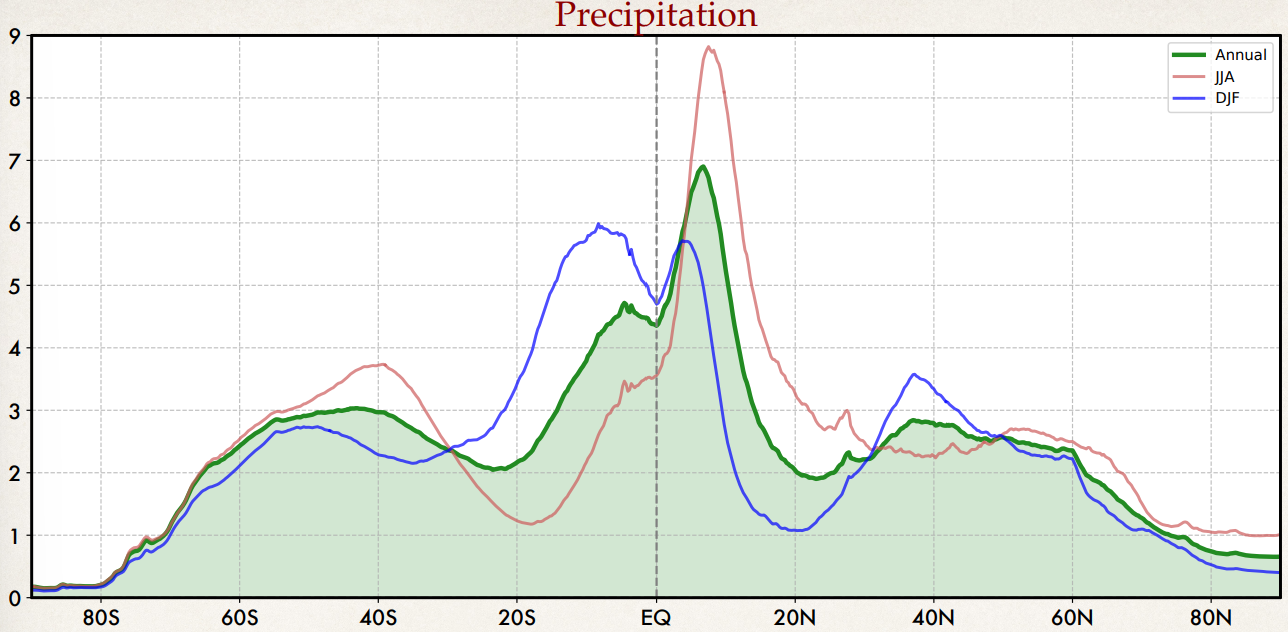
\includegraphics[width=0.5\linewidth]{uploads/precipit.png}
	\caption{Latitudinal distribution of precipitation for Annual
		mean and Seasonal Cycle. Units are mm/day}
	\label{fig:enter-label}
\end{figure}
SLIDE 8-9 AUDIO
However interesting things happen when the heating varies in x, and it is localized as the observation of precipitation shows. The precipitation in the mid-latitude is aligned along the preferred path of developing storms, the storm tracks. This precipitation is due to the rising of warm, moist air due to the baroclinic instabilities in the westerly current of the mid-latitudes. Precipitation linked to the baroclinic storm tracks in Winter can be seen from the East coast of North America elongating into Europe and the Mediterranean and from the Asian Far East into the Pacific Ocean. The Summer monsoonal precipitations of the South Asian Monsoon over India and Indochina, of the West Africa Monsoon, and of the weaker North American Monsoon are clearly visible. In general, major convective centers are present over South America and over the Maritime Continent.


An idealized case can be given by
\begin{figure}[htp!]
	\centering
	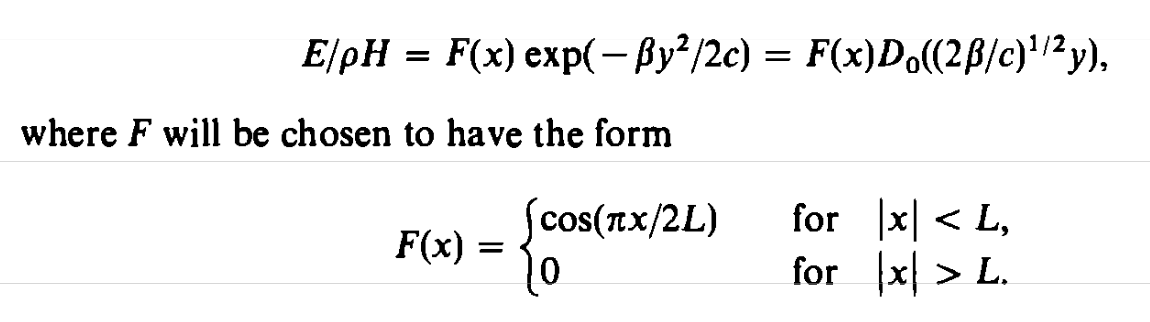
\includegraphics[width=0.5\linewidth]{uploads/22image.png}
	\label{fig:enter-label}
\end{figure}

What about if I assume a basic state, meaning a rest atmosphere, and do the same operations as before? Imposing specific boundary conditions led us to a kinematic condition telling us that if air is heating near a mountain, this air does not go inside the mountain but the flow will go above it. This phenomenon stresses that mountains are a steady source of vorticity.

AUDIO 33'

In 1979 Grose and Hoskins published a paper describing an investigation that has been conducted of the steady response to orography as described by the linearized shallow-water equations on the sphere.
Results have been obtained for both idealized and realistic climatological mean zonal flows when perturbed by simple isolated mountains.

\begin{figure}[htp!]
	\centering
	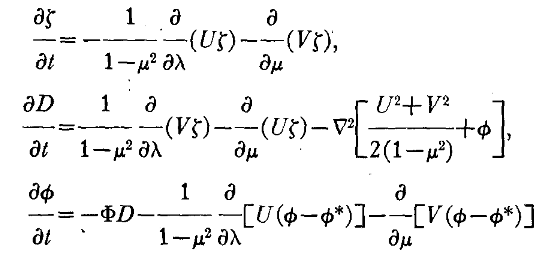
\includegraphics[width=0.5\linewidth]{uploads/19image.png}
	\caption{Equations on the sphere}
	\label{fig: fig 2.2}

\end{figure}
where $\zeta$ is the absolute vorticity, D the divergence, $\Phi$
the average height of the fluid multiplied by the gravitational constant g, $\varphi$ the deviation of the free surface from that height multiplied by g and $\varphi^*$ the height of the orography multiplied by g. The latitude and longitude are denoted by $\theta$ and $\lambda$ with $\mu = \sin \theta$. The variables U and V are respectively the zonal and the meridional velocities multiplied by $\cos \theta$.


The two scientists want to transform equations in Figure \ref{fig: fig 2.1} in a steady state, to have it they need forcing (external from the system and not described dynamically) and they have to eliminate the time derivative substituting it with the dissipative term.
In particular, the forcing here is represented by $\varphi^*$ because scientists arbitrarily impose it.
AUDIO 48' POMEE




\subsection{What is the mechanism by which SST is affecting climate?}

Sea Surface Temperature (SST) plays a critical role in shaping long-term climate variability, particularly on timescales beyond weeks (synoptic timescales), where its influence on atmospheric circulation becomes pronounced. Unlike land surfaces, which adjust quickly to temperature changes and lack long-term memory, the ocean's thermal inertia allows SST to maintain a prolonged impact on the climate system (the rate of change of $T$ is the resulting balance of heat emission). On land, soil moisture provides a limited form of memory, influencing land-atmosphere interactions for up to a year, but the ocean’s capacity to modulate heat exchange and atmospheric patterns makes its effect far more persistent and complex.

The mechanism by which SST affects the atmosphere primarily involves vorticity balance, a key dynamic in atmospheric motion. In equatorial regions, SST anomalies act as localized heating sources, driving convection that alters circulation patterns. When heating occurs, air rises, leading to asymmetrical atmospheric responses in the east-west direction. This localized heating produces cyclonic activity in the lower atmosphere and upper-level vortices displaced from the heating source due to atmospheric dynamics. Localized heating from SST causes air to rise, which in turn generates cyclonic and anticyclonic vortices at different atmospheric levels.  These processes demonstrate how SST anomalies force changes in atmospheric circulation, influencing phenomena such as tropical cyclones, monsoons, and large-scale weather patterns.

\begin{figure}[htp!]
	\centering
	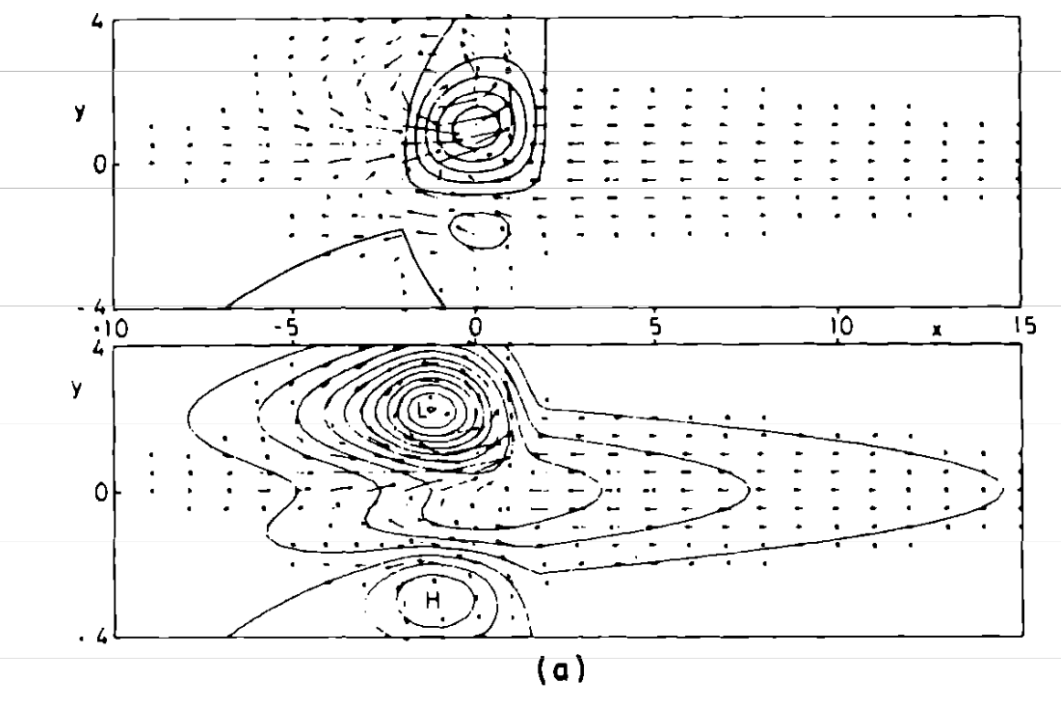
\includegraphics[width=0.4\linewidth]{uploads/Screenshot 2024-11-26 100719.png}
	\caption{Schematic of atmospheric circulation that exhibits cyclonic asymmetry.}
	\label{fig:enter-label}
\end{figure}



In the figure above, the contours represent streamlines or geopotential height isolines in the upper atmosphere, while vectors show wind flow pattern. The cyclonic circulation (low-pressure system "$L$") indicates counterclockwise motion in the NH. The pattern is asymmetrical meaning that the cyclonic core does not produce perfeclty concentric circulation due to asymmetries in forcing. In the high-pressure region "$H$", the arrows and contours suggest a wave-like structure extending downstream of the low-pressure system, representing possibly Rossby waves generated by heating or perturbation. Note that the generation of vorticity in the lower and upper layers may have opposite signs.



In simplified models of atmospheric circulation, such as a barotropic system with constant wind and dissipation, external forcing like heating or topography alters the basic state. Dissipation, including radiative cooling, ensures that the energy added to the system by these forcings does not lead to instability, allowing for a stationary solution. Remember Grose and Hoskins illustrate how mountains can generate Rossby waves, which are planetary-scale atmospheric waves that propagate and redistribute energy and momentum. These waves, influenced by both topographic features and SST anomalies, play a significant role in driving global circulation patterns, such as the jet stream and climate anomalies.

The adjustment to forcing is more challenging over oceans than land because of the ocean’s slower response time. SST anomalies serve as a sustained forcing mechanism, particularly in tropical regions, driving long-term changes in atmospheric circulation through convection and vorticity dynamics. By generating Rossby waves and other large-scale atmospheric responses, SST anomalies influence both local weather events and global climate patterns. This intricate coupling between ocean and atmosphere underscores the importance of SST in understanding and predicting long-term climate variability.\\[0.25 cm]

\subsection{Steady heating balances}
\textbf{Hoskins and Karoly}\cite{Hos81} (1981) investigated the atmospheric response to stationary heating using a General Circulation Model (GCM) with a realistic structure. Their approach involved simplifying a complex mathematical system by linearizing the model. The focus was on understanding the stationary solutions that arise from this linearized problem.

To explore the response to heating, they used discretization methods. This involves breaking down the atmosphere into grid points or using spectral resolution. For example, with a grid resolution of 2 degrees, there are approximately 18000 points (calculated as $180/2×360/2$), and if the model has 9 vertical levels ($\rightarrow$ Manabe), this results in 162,000 unknowns. Solving such a system requires constructing a matrix $\mathbf{A}$, with dimensions based on the degrees of freedom, and then solving the linear equation $\mathbf{A}\mathbf{x}=\mathbf{f}$, where
$\mathbf{x}$ represents the variables of interest, and $\mathbf{f}$ is the forcing vector.

However, directly constructing and solving such a massive matrix is computationally intensive. An alternative approach is to use the model itself, where the prognostic equations are represented as $\mathbf{\dot{x}}=\mathbf{F(x)}$. Adding a heating term $Q$, this becomes $\mathbf{\dot{x}=F(x)}+Q$, since $\mathbf{F(x)}$ is nonlinear, linearization is required to solve for perturbations. By introducing a small perturbation $\mathbf{x'}$ at one grid point: $\mathbf{x=\overline{x}+x'}$, where $\mathbf{x'}$  is structured as a special vector (e.g., $[1,0,0,\dots]$, the model’s response provides the derivative of $\mathbf{F}$ that is just the basic state $\mathbf{\dot{x}=\dot{\overline{x}}}$, forming a i-column of $\mathbf{A}$, corresponding to the position of $1$ in the special perturbation vector. Repeating this process for all degrees of freedom (grid points or spectral coefficients of divergence, vorticity, ... depending on which discretization model you use) constructs the entire matrix.

\paragraph{Balancing heating and advection.}
Let's look at the balances in the thermodynamical equation.
\begin{align}
	\overline{u}\frac{\partial\theta}{\partial x}+{v}\frac{\partial\overline{\theta}}{\partial y}+w\frac{\partial\overline{\theta}}{\partial z}=Q \\
	f\overline{u}\frac{\partial v}{\partial x}-f{v}\frac{\partial\overline{u}}{\partial z}+wN^2=Q
\end{align}
means:
\begin{figure}[htp!]
	\centering
	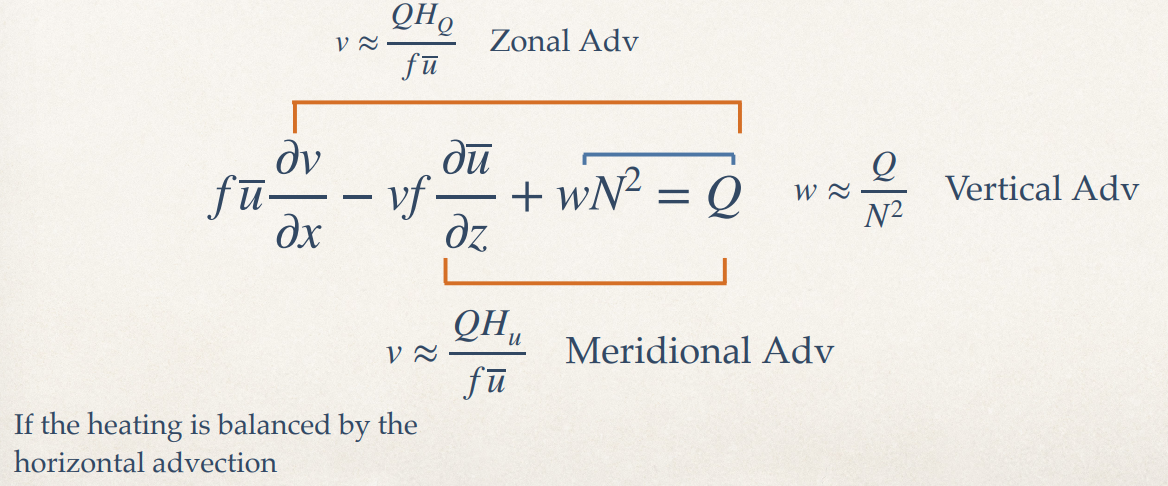
\includegraphics[width=0.5\linewidth]{uploads/Screenshot 2024-11-26 104817.png}
	\caption{heat balance}
	\label{fig:enter-label}
\end{figure}

In the vertical advection case then the vorticity balance is between the beta terms and the stretching term:
$$\beta v\approx fx_z=\frac{fQ}{N^2H_Q}$$
The mechanism with smaller v will dominate, the horizontal advection are of the form:
$$v\approx\frac{QH}{f\overline{u}}$$
and the vertical:
$$v\approx\frac{Q}{N^2}$$
so the dominant process is given by
\begin{equation}
	\gamma=\frac{f\overline{u}^2}{\beta N^2HH_Q}
\end{equation}
Horizontal advection will dominate for small $H_Q$, vertical
advection otherwise. Depending of the size of $\gamma$ heating will balanced by horizontal advection if $\gamma \gg 1$ and by vertical advection if $\gamma\ll 1$.
In the tropics $\gamma$ is small if $H_Q$ is greater than 1 km, so any heating near the surface will generate large meridional motions, but heating away from the surface will generate vertical motions.
\begin{figure}[htp!]
	\centering
	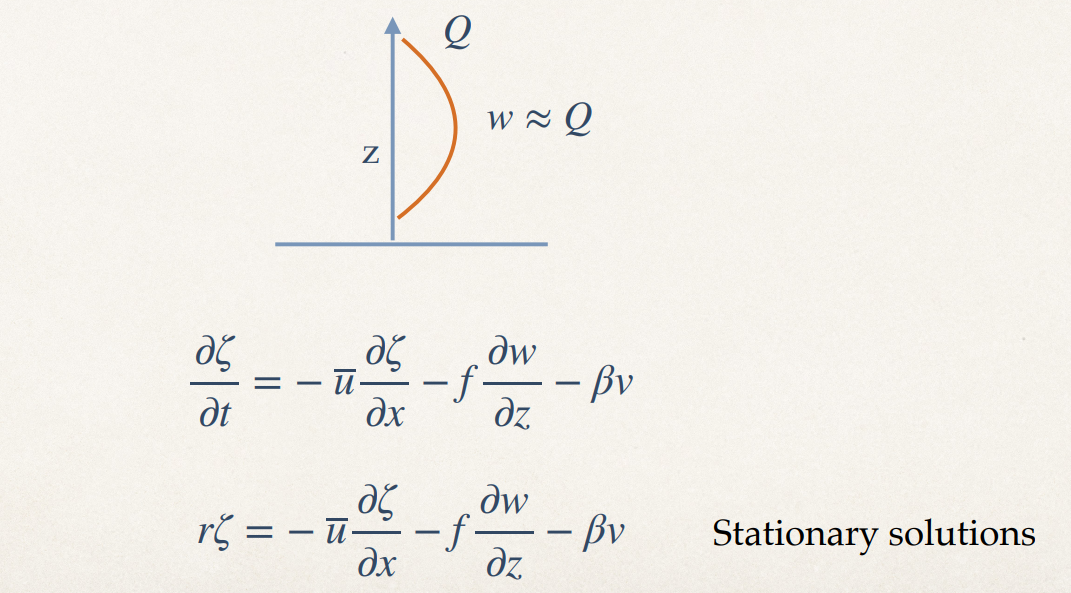
\includegraphics[width=0.5\linewidth]{uploads/Screenshot 2024-11-26 105240.png}
	\caption{Heating and vertical motion}
	\label{fig:enter-label}
\end{figure}


The heating induced by processes like deep convection leads to vertical or horizontal advection, but the dominant mechanism depends on factors such as the stratification of the atmosphere and the strength of the Coriolis parameter. The competition between vertical and horizontal advection can be quantified by a parameter $\gamma$, which helps determine which process dominates, the mechanism generating the smaller advection will dominate as it's easier to treat. In equatorial regions, where SST exceeds 28.5°C, strong deep convection generates significant vertical motion, impacting the overall circulation.

\paragraph{Vorticity balances and responses to heating}
Heating anomalies, such as those driven by SST, lead to vorticity generation with distinct impacts depending on the region. In the tropics, heating often induces vertical motion and deep convection, while in extratropical regions like the North Atlantic, the vorticity balance is more complex due to baroclinic and barotropic processes. Heating anomalies result in opposite vorticity generation in upper and lower layers, with vertical stratification and horizontal advection playing critical roles.

The implications of anomalous heating differ significantly between regions. For instance, in the North Atlantic, heating anomalies can produce teleconnections, altering large-scale circulation patterns over several months. These teleconnections, resembling the findings of Horace and Wallace on SST variability, highlight how localized heating can influence global atmospheric dynamics.
\begin{figure}[htp!]
	\centering
	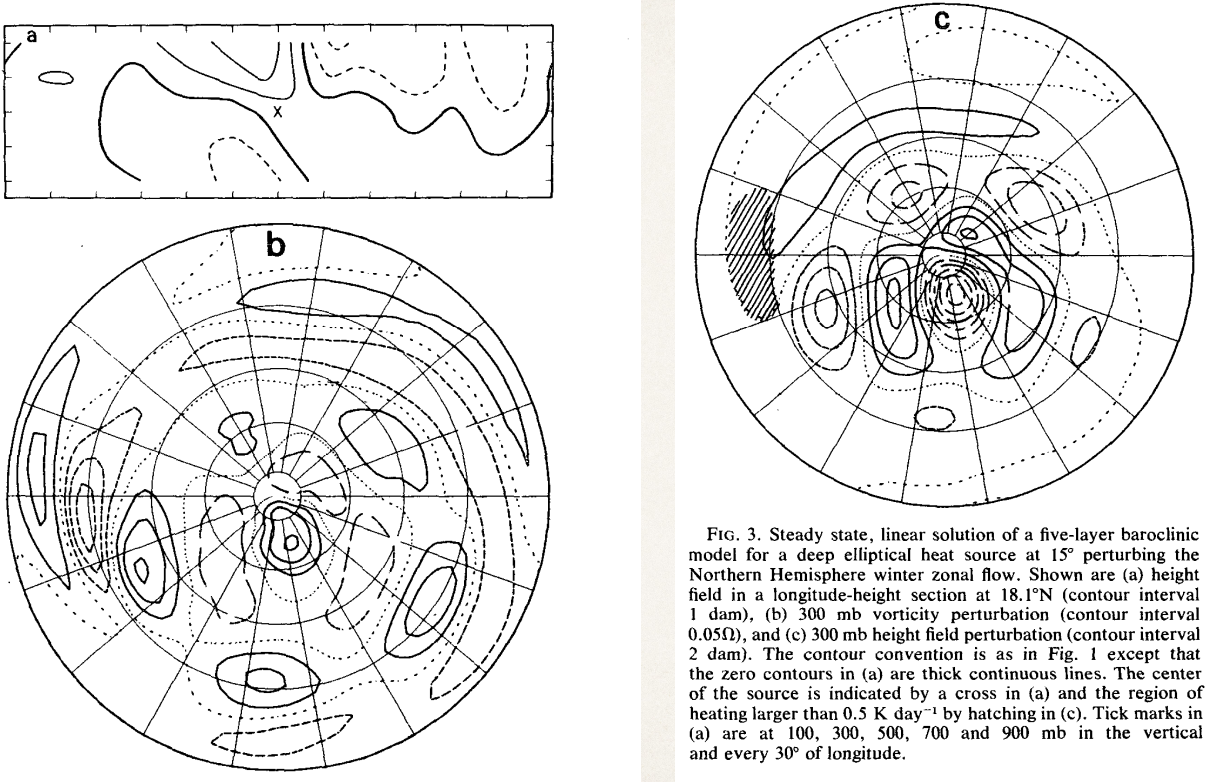
\includegraphics[width=0.4\linewidth]{uploads/Screenshot 2024-11-26 104358.png}
	\caption{steady-state, linear solution of a five-layer baroclinic model.}
	\label{fig:enter-label}
\end{figure}

Teleconnections, or long-distance climate influences, can arise from dynamical causes over intermediate timescales (e.g., months). They are often linked to SST variability and heating-induced circulation changes. However, the assumption of a simple atmospheric basic state limits these analyses because real-world atmospheric states are far more complex.

Atmospheric anomalies tend to grow along gradients, where temperature or pressure contrasts enhance the instability and amplify the response to heating. This gradient-based growth underpins many of the patterns observed in teleconnections and regional responses to SST anomalies.
\\
[0.2cm]

Differences in SST can significantly influence atmospheric processes. Variation in SST can lead to extra convection and extra precipitation (particularly in regions where the ocean surface warms beyond certain thresholds that enhance evaporation and moisture availability). When these responses are systematic and persistent over time, they can act as a form of external forcing on the atmosphere, triggering large-scale atmospheric patterns. These responses can resempble \textbf{Rossby waves patterns}\footnote{large scale atm waves resulting from conservation of vorticity in the presence of Earth's rotation and varying lat}.

\begin{figure}[htpb]
	\centering
	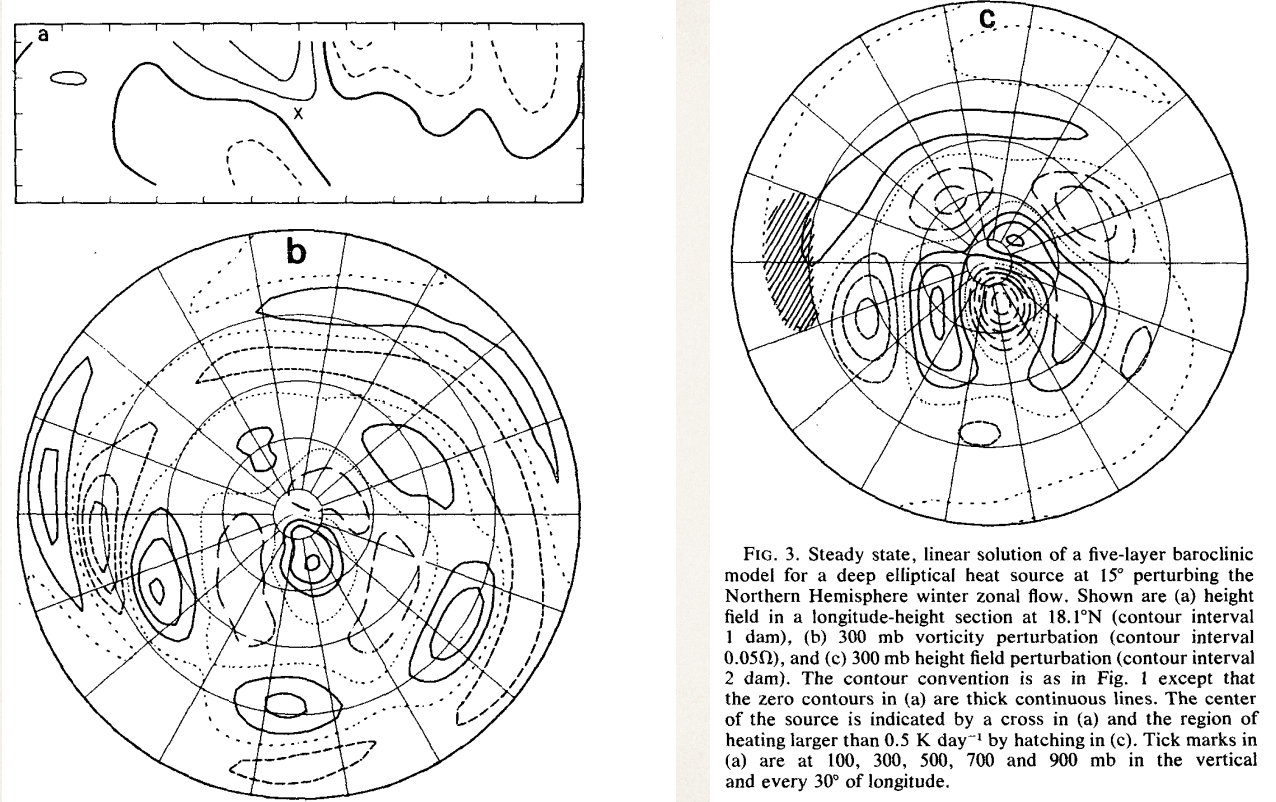
\includegraphics[width=0.5\linewidth]{uploads/imagewavesconn.png}
	\caption{systematic SST-induced convection can produce predictable atmospheric wave patterns.}
	\label{fig:enter-label}
\end{figure}
\paragraph{Atmpsphere behaviour: linear or non-linear?}
A key question in atmospheric science is whether the atmosphere behaves linearly or nonlinearly. For synoptic-scale phenomena (timescales of days/weeks), the atmosphere operates in in a highly nonlinear regime, with chaotic dynamics dominating the system's behavior. At longer timescales, when averaged over months or seasons, the system can exhibit more predictable patterns. By focusing on time-mean states, the attempt is to determine whether atmospheric responses to SST variability, which manifest as anomalies, are linear or nonlinear. This remains a topic of active debate, as atmospheric anomalies often exhibit behaviors influenced by both linear responses to forcing and nonlinear interactions within the system.
\\[0.2 cm]

Rowell (1995)\cite{Ross95} highlighted the potential for increased atmospheric predictability by exploiting SST data. From Lorenz's work, which identified the chaotic nature of atmospheric dynamics and the inherent predictability limits (two weeks for weather forecasting), Rowell built the concept of \textbf{potential predictability}, which measures how strongly SST anomalies influence atmospheric conditions ("potential" indicates that this also depends on predictions of
anomalous oceanic forcing). The argument is that if SSTs can be accurately predicted over longer periods, such as months, they can serve as a boundary forcing for the atmosphere, enabling predictions of atmospheric anomalies on similar timescales. \\
Rowell focused on estimating the potential seasonal predictability of the atmosphere by analyzing results from a General Circulation Model ensemble over multiple decades. His work aimed to determine how well atmospheric anomalies could be predicted when SST variability was used as a forcing mechanism. \\



The atmosphere behaves as a chaotic system and as a consequence, deterministic predictability is limited.
However, it is also well known that at many locations, predictability of seasonal weather statistics is also
possible. This arises from what may be termed ‘‘external’’ factors that alter the likelihood of residence in
atmospheric attractors, enabling probabilistic forecasts to be made of the seasonal mean state, on
condition that the external forcing is itself predictable.
The primary source of such external forcing at seasonal timescales arises from sea surface temperature
(SST) patterns; these can indeed be predicted, either using coupled dynamical models (e.g., Cane et al.
1986; Barnston et al. 1994; Ji et al. 1994) or statistical models (e.g., Ward et al. 1993; Barnston et al. 1994).
It is clearly important to be able to assess where on the globe atmospheric variations are sufciently
affected by oceanic forcing to enable practical seasonal prediction. This requires measurements of
atmospheric potential predictability.

\paragraph{Potential predictability} The atmosphere-ocean system exhibits two main types of variability:
\begin{enumerate}
	\item \textbf{Internal variability}, arising from the internal dynamics of the coupled system as a fluid system, such as turbulence, convection, and other processes within the fluid dynamics framework.
	\item \textbf{External variability}, which is the response of the system to external forcing, such as changes in SST, solar radiation, or anthropogenic influences.
\end{enumerate}
In the context of SST-driven atmospheric anomalies, SST serves as an external forcing mechanism, potentially providing a source of predictability. This raises the question: How strongly does SST variability influence atmospheric anomalies? The strength of this influence determines the degree of potential predictability.\\

If the control exerted by SST on atmospheric anomalies is strong, then accurate SST predictions would lead to a high degree of atmospheric predictability. This concept can be broken into two components:
\begin{enumerate}
	\item Internal response: The portion of atmospheric variability that would occur regardless of whether SST varies or remains constant.
	\item External response: the portion of atmospheric variability driven directly by SST changes over time.
\end{enumerate}
undertanding these two components, science can evaluate the relative influence of SST as a boundary forcing mechanism and check the limits of atmospheric predictability in the context of cliamte modeling. \\


Rowell's study confirmed that SST anomalies have a significant impact on seasonal atmospheric predictability. It highlighted that large-scale, systematic SST patterns (e.g. those associated with El Niño-Southern Oscillation, or ENSO) create atmospheric responses that can dominate the external variability signal.
SST-driven predictability varies across regions and seasons:
\begin{itemize}
	\item tropical regions show higher predictability due to strong ocean-atm coupling, particularly in areas influenced by ENSO events.
	\item Mid-latitudes have weaker and less consistent predictability because atm dynamics in these regions are dominated by internal variability
\end{itemize}
Hence, accurate SST predictions could allow for better forecasting of atmospheric anomalies, especially in regions where SST strongly influences weather patterns.\\
[0.2cm]


Potential variability examines how much of the total variance in a climate model can be explained by external forcing versus the system's intrinsic chaotic behavior. If the system is insensitive to external forcing, such as prescribed SST, even perfect SST predictions would not yield meaningful atmospheric predictions. Therefore, a robust analysis is required to separate and quantify these components. A statistical technique, ANOVA is used to partition the variance in the system into components associated with external forcing and internal variability. By analyzing the ensemble simulations, ANOVA helps determine the sensitivity of the atmosphere to SST forcing and distinguishes between variance arising from the chaotic nature of the system and variance driven by external boundary conditions.
\paragraph{ANOVA} The ensemble simulations will provide time series of data in $(n+2)$ dimension, if $n$ is
the dimension of the geographical labels. For instance, considering atmospheric variables at a single level will result in data labeled by (latitude, longitude, time, ensemble index). The data can be further aggregated using averages to the level necessary for the analysis, in most cases monthly means are the primary data sets. The objective is to separate the total variance $\sigma^2_{TOT}$ in the component caused by the external forcing (SST) and the system at rest:
$$\sigma_{TOT}^2=\sigma^2_{SST}+\sigma^2_{INT}$$
Imagine that data are available from an ensemble of n climate
simulations, each of $N$ years in length, each forced by the same
varying SSTs and sea ice, and each one differing from the others only
by its initial atmospheric conditions. Consider a characteristic, X, which can be quantied for each individual season, for example, the time mean of some variable at a point, a higher moment statistic, a regional index, or an EOF time coefficient.
$$x_{ij}=\mu_i+\epsilon_{ij}$$
By averaging across ensemble members for each grid point, high-frequency fluctuations are smoothed out. This process retains only the components of variability common across ensembles, isolating the SST-forced response. At each grid point, the average of the ensemble realizations represents the SST-forced mean, $\mu_i$, which varies across grid points. The variance of the ensemble mean over time reflects the contribution of SST variability to the total system variability.

To explore how the climate system responds to external forcing and check variability, ensemble simulations are critical, and they can be done in different ways:
\begin{enumerate}
	\item with the same SST forcing: multiple ensamble are run with identical prescribed SSTs to analyze the system's response. While all simulations "see" the same SSTs, their responses will differ due to the chaotic nature of the atmosphere. These differences help isolate internal variability.
	\item with different initial conditions: each ensemble starts with different i.c., leading to divergent evolutions over time even if they are subject to the same SST boudary conditions.
	\item with separated internal and external variability
\end{enumerate}
Using a single model for these ensembles relies heavily on the model's accuracy and assumptions. Errors or biases inherent in the model could compromise the reliability of the analysis.
To mitigate this, multi-model ensembles are increasingly used. These involve simulations from various climate models, reducing the dependency on any single model's characteristics and providing a more robust estimate of externally forced variability. \\

If the atmospheric response to SST forcing is weak or highly chaotic, predictability is inherently limited, even with perfect knowledge of future SSTs.
Conversely, a strong and consistent atmospheric response to SSTs suggests higher potential predictability, emphasizing the importance of accurately predicting SSTs for reliable seasonal or interannual atmospheric forecasts.

The exploration of ensemble simulations, combined with tools like ANOVA, forms the basis for understanding the sensitivity of the climate system to external forcing and quantifying the relative contributions of internal and external variability. By systematically prescribing SSTs and analyzing the spread of ensemble responses, researchers can assess the potential predictability of atmospheric phenomena while addressing the chaotic nature of the system.






the idea is the following: two ensembles
\begin{itemize}
	\item A statistical technique ANOVA ("analysis of variance")
	\item Exploit sensitivity of the climate system to generate ensambles of simulation with the same £external" forcing, i.e. prescribed SST.
	\item Relies on skill on a single model
	\item late, use many models
\end{itemize}


The ratio of SST variance to total variance provides a measure of potential predictability, hence indicates the system's sensitivity to SST variations. If the ratio approaches 1, most of the system's variability is controlled by SST forcing.
\begin{equation}\label{eq.pot predictability}
	\rho=\frac{\sigma^2_{SST}}{\sigma^2_{TOT}}
\end{equation}

\paragraph{Predictability across regions}
\begin{itemize}
	\item Tropical regions: SST has strong control over tropical precipitation variability.
	      The ensemble mean explains a significant portion of the variance, indicating that SST-forced variability dominates. For example tropical precipitation anomalies respond robustly to SST changes, and this relationship is crucial for understanding heat distribution in the climate system.
	\item Mid-latitudes: the relationship between SST and precipitation variability becomes weaker, and the system exhibits greater internal variability.
	      Heat anomalies driven by precipitation in the tropics can influence mid-latitudes, as seen in the Hoskins and Currie results. However, the predictability is less robust in these regions.
\end{itemize}

\paragraph{Challenges in observations}
Observations provide only one realization of the climate system, unlike models that allow for ensemble simulations. This limitation makes it challenging to disentangle forced variability from internal variability directly. Monthly time series of observed SST can provide a proxy for estimating SST-forced variability but lack the direct ability to separate components of variance as in ensemble modeling.\\




Potential predictability can be visualized as the fraction of variance explained by SST across all grid points, normalized to range between 0 and 1. This measure shows \ref{fig:potpred}: strong potential predictability in the tropics, where SST controls much of the variance in upper-layer variables.
Weak potential predictability in mid-latitudes, reflecting greater internal variability and weaker SST control.

\begin{figure}[htpb]
	\centering
	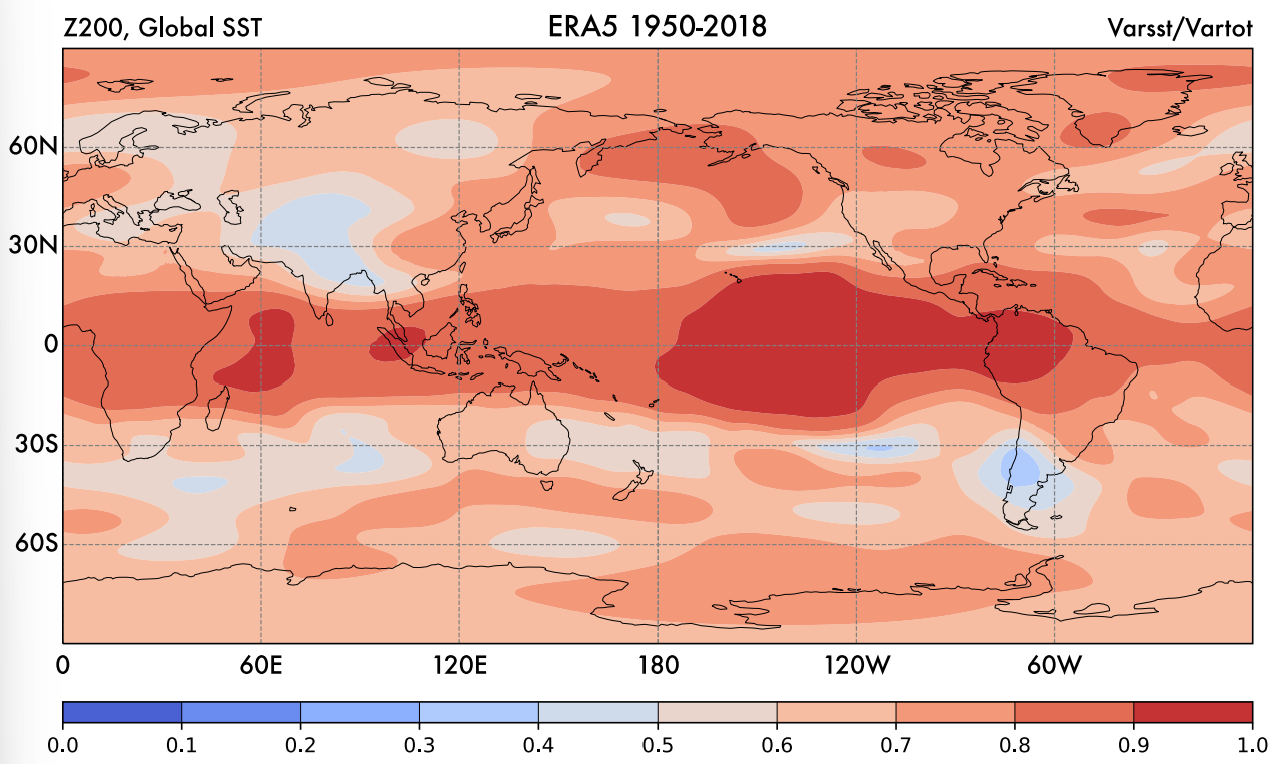
\includegraphics[width=0.5\linewidth]{uploads/potpred.png}
	\caption{Potential predictability as the fraction of variance explained by SST across all grid points.}
	\label{fig:potpred}
\end{figure}











In mid-latitudes variability is harder to predict due to a weaker direct SST influence and a more dominant role of internal dynamics. Monsoonal circulations while influenced by SST variability, they are not entirely governed by it. Their predictability is thus less robust than tropical SST-forced responses.

Understanding the relative contributions of SST and internal variability is critical for seasonal climate predictions.
The strong control of tropical SST over precipitation anomalies offers promising avenues for prediction, especially in the tropics, whereas mid-latitudes remain more uncertain.


Using ANOVA and ensemble simulations, researchers can assess the sensitivity of the climate system to SST forcing. The ratio of SST variance to total variance serves as a measure of potential predictability, which is higher in the tropics due to the strong SST-precipitation coupling and decreases in mid-latitudes due to greater internal variability. This understanding is foundational for improving seasonal climate predictions and exploring the dynamics of coupled ocean-atmosphere systems.



